%%%%%%%%%%%%%%%%%%%%%%%%
%%%% DOCUMENT START %%%%
%%%%%%%%%%%%%%%%%%%%%%%%

\documentclass[10pt]{article}
\usepackage{graphicx,url}
\usepackage[utf8]{inputenc}  

\usepackage[T1]{fontenc}
\usepackage{xcolor}

\usepackage{listings}
\renewcommand{\lstlistingname}{Query}
\lstset{
    language=SQL,
    basicstyle=\ttfamily\small,
    numbers=left,
    numberstyle=\tiny\color{gray},
    keywordstyle=\color{blue}\bfseries,
    commentstyle=\color{green!40!black},
    stringstyle=\color{red!70!black},
    frame=single,
    breaklines=true,
    showstringspaces=false,
    captionpos=b
}


\usepackage{csvsimple}
\usepackage{caption}
\usepackage{adjustbox}
     

\sloppy

\title{\vspace{-2em}Trabalho Final — Querries}
\date{}
\author{
    Douglas C. de Carvalho\\
    \small Faculdade de Engenharia -- Departamento de Engenharia de Sistemas e Computação\\
    \small Universidade do Estado do Rio de Janeiro (UERJ) -- Rio de Janeiro -- RJ -- Brasil\\
    \small \texttt{github.com/d0ugcarv/projeto\_final\_mapeia\_verde}
}


\begin{document}
    \maketitle

    \section*{Módulo 3 (Consultas Básicas)}

    \lstinputlisting[
        language=SQL,
        caption={Exemplo de Consultas Básicas},
        label={query:modulo_3}
    ]{querries/modulo_3_consultas_basicas.sql}

    \begin{figure}[htbp]
        \centering
        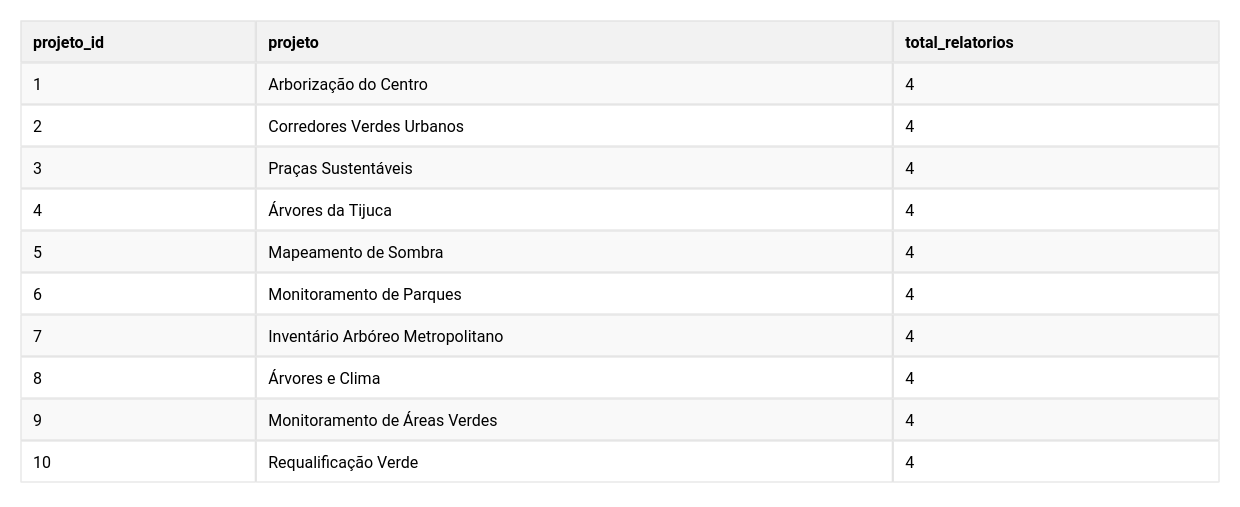
\includegraphics[
            width=\textwidth,
            height=0.8\textheight,
            keepaspectratio]
            {querries_images/modulo_3_consultas_basicas.png}
        \caption{Tabela gerada com a query}
        \label{fig:consultas_basicas_modulo_3}
    \end{figure}


    \clearpage
    \section*{Módulo 4 (Filtros)}

    \lstinputlisting[
        language=SQL,
        caption={Exemplo de Filtros},
        label={query:modulo_4}
    ]{querries/modulo_4_filtro.sql}

    \begin{figure}[htbp]
        \centering
        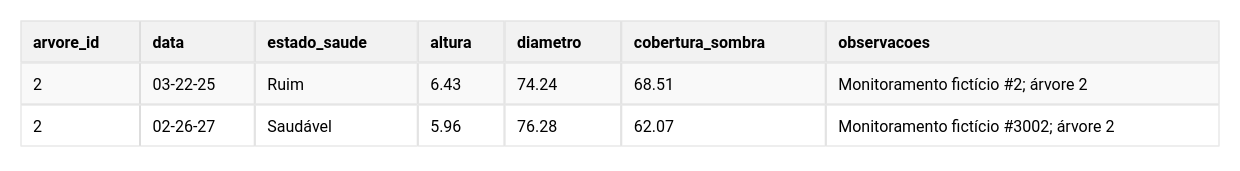
\includegraphics[
            width=\textwidth,
            height=0.8\textheight,
            keepaspectratio]
            {querries_images/modulo_4_filtro.png}
        \caption{Tabela gerada com a query}
        \label{fig:consultas_basicas_modulo_4}
    \end{figure}


    \clearpage
    \section*{Módulo 5 (Operações Básicas e Agregação)}

    \lstinputlisting[
        language=SQL,
        caption={Exemplo de Operações Básicas e Agregação},
        label={query:modulo_5}
    ]{querries/modulo_5_operacoes_basicas_e_agregacao.sql}

    \begin{figure}[htbp]
        \centering
        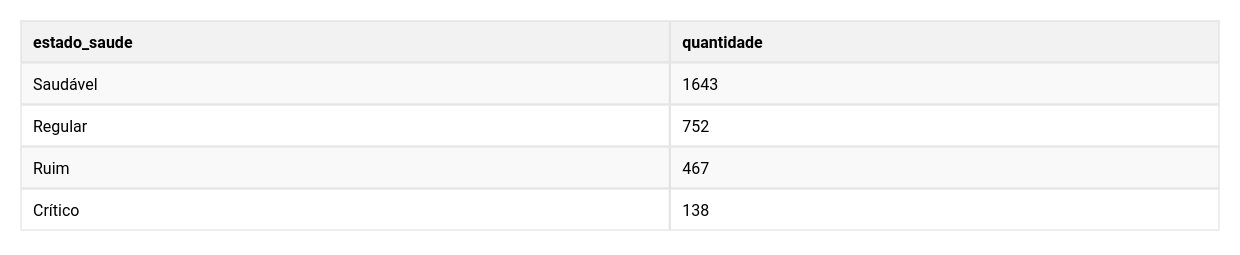
\includegraphics[
            width=\textwidth,
            height=0.8\textheight,
            keepaspectratio]
            {querries_images/modulo_5_operacoes_basicas_e_agregacao.png}
        \caption{Tabela gerada com a query}
        \label{fig:consultas_basicas_modulo_5}
    \end{figure}



    \clearpage
    \section*{Módulo 6 (Agrupamentos)}

    \lstinputlisting[
        language=SQL,
        caption={Exemplo de Agrupamentos},
        label={query:modulo_6}
    ]{querries/modulo_6_agrupamentos.sql}

    \begin{figure}[htbp]
        \centering
        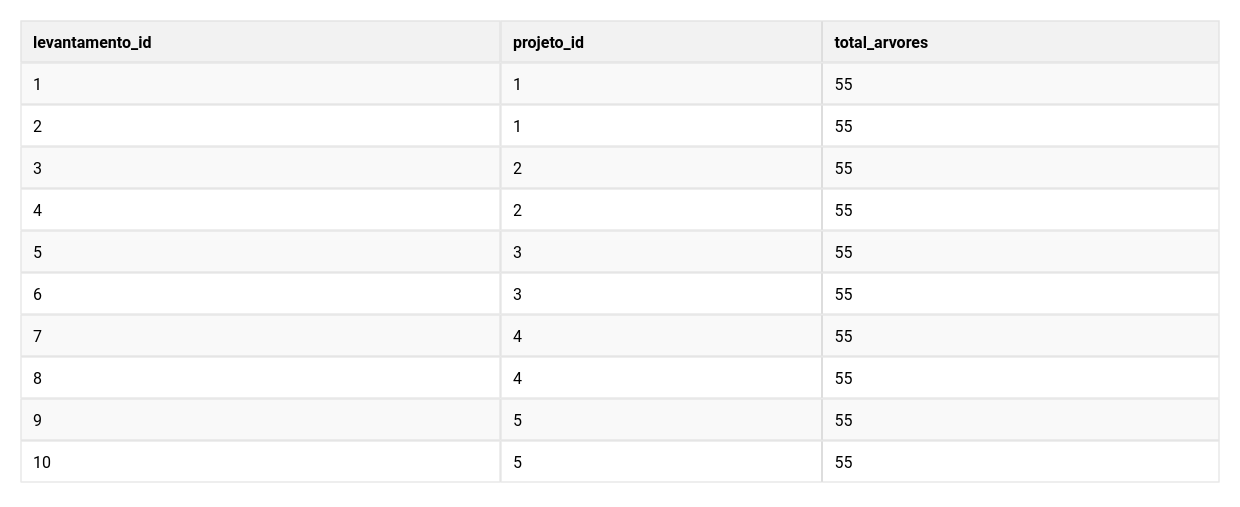
\includegraphics[
            width=\textwidth,
            height=0.5\textheight,
            keepaspectratio]
            {querries_images/modulo_6_agrupamentos.png}
        \caption{Tabela gerada com a query}
        \label{fig:consultas_basicas_modulo_6}
    \end{figure}



    \clearpage
    \section*{Módulo 7 (Variáveis e CAST)}

    \lstinputlisting[
        language=SQL,
        basicstyle=\ttfamily\tiny,
        caption={Exemplo de Variáveis e CAST},
        label={query:modulo_7}
    ]{querries/modulo_7_variaveis_e_cast.sql}

    \begin{figure}[htbp]
        \centering
        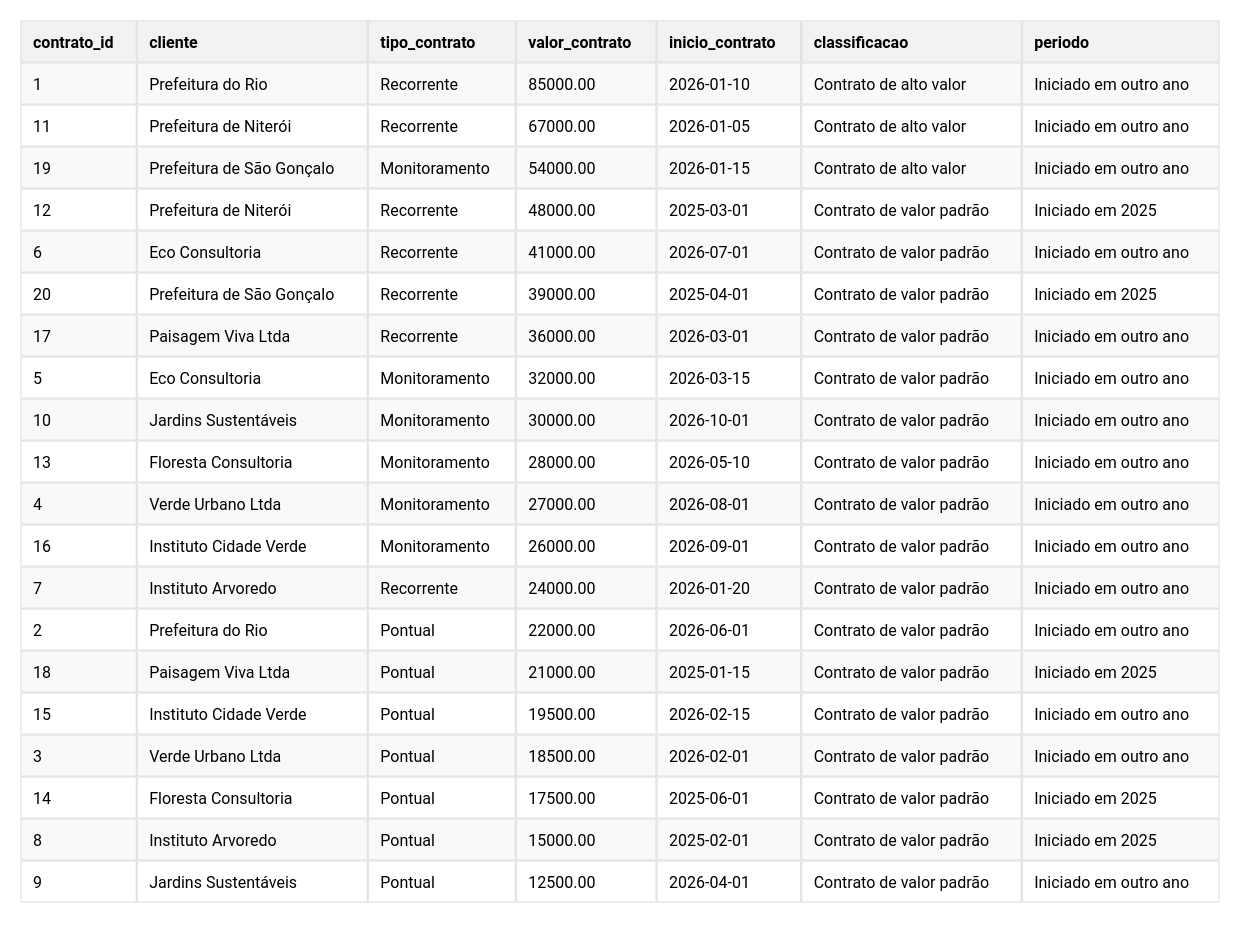
\includegraphics[
            width=\textwidth,
            height=0.4\textheight,
            keepaspectratio]
            {querries_images/modulo_7_variaveis_e_cast.png}
        \caption{Tabela gerada com a query}
        \label{fig:consultas_basicas_modulo_7}
    \end{figure}



    \clearpage
    \section*{Módulo 8 (Funções de Texto e Data)}

    \lstinputlisting[
        language=SQL,
        basicstyle=\ttfamily\tiny,
        caption={Exemplo de Funções de Texto e Data},
        label={query:modulo_8}
    ]{querries/modulo_8_funcoes_de_texto_e_data.sql}

    \begin{figure}[htbp]
        \centering
        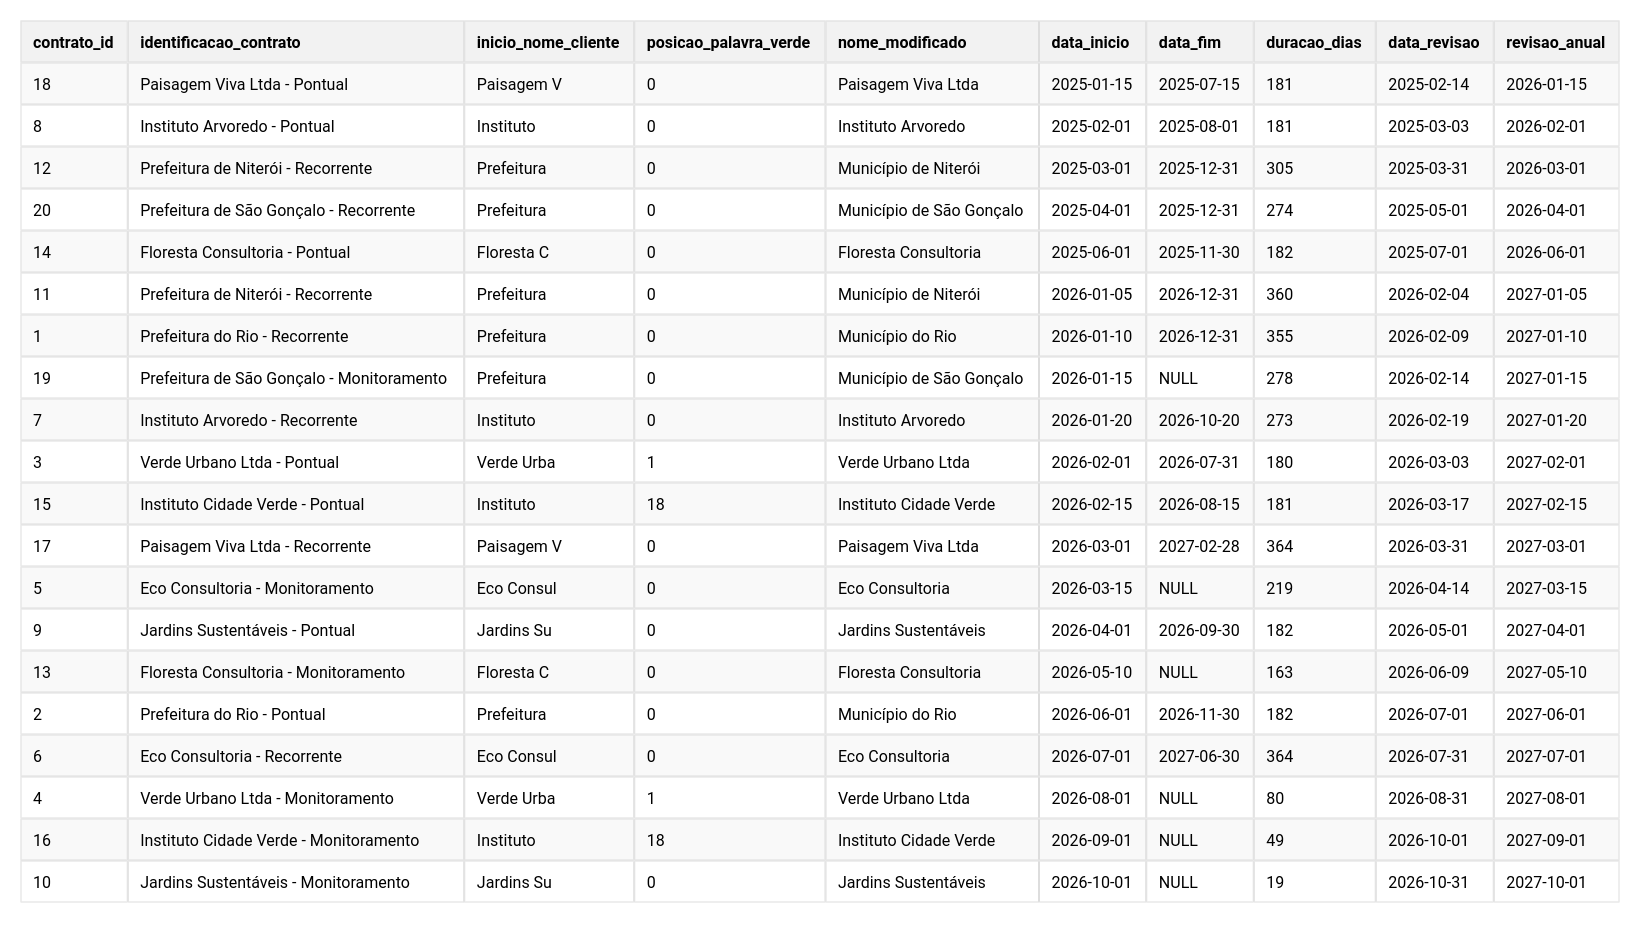
\includegraphics[
            width=\textwidth,
            height=0.25\textheight,
            keepaspectratio]
            {querries_images/modulo_8_funcoes_de_texto_e_data.png}
        \caption{Tabela gerada com a query}
        \label{fig:consultas_basicas_modulo_8}
    \end{figure}



    \clearpage
    \section*{Módulo 9 (JOINs e Relacionamentos)}

    \lstinputlisting[
        language=SQL,
        caption={Exemplo de JOINs e Relacionamentos},
        label={query:modulo_9}
    ]{querries/modulo_9_joins_e_relacionamentos.sql}

    \begin{figure}[htbp]
        \centering
        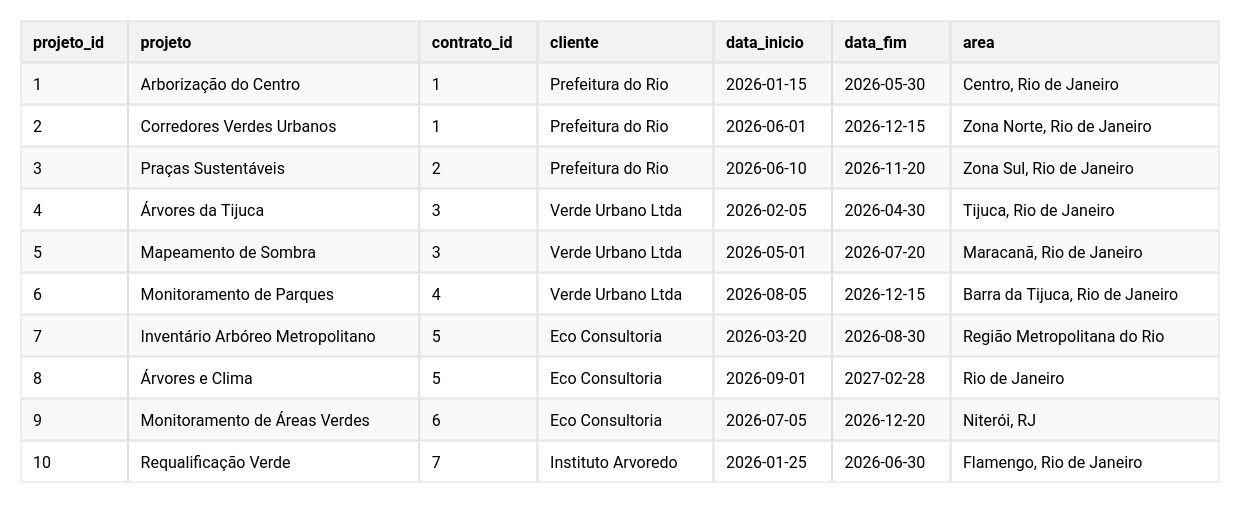
\includegraphics[
            width=\textwidth,
            height=0.8\textheight,
            keepaspectratio]
            {querries_images/modulo_9_joins_e_relacionamentos.png}
        \caption{Tabela gerada com a query}
        \label{fig:consultas_basicas_modulo_9}
    \end{figure}



    \clearpage
    \section*{Módulo 10 (Funções Condicionais)}

    \lstinputlisting[
        language=SQL,
        basicstyle=\ttfamily\tiny,
        caption={Exemplo de Funções Condicionais},
        label={query:modulo_10}
    ]{querries/modulo_10_funcao_condicionais.sql}

    \begin{figure}[htbp]
        \centering
        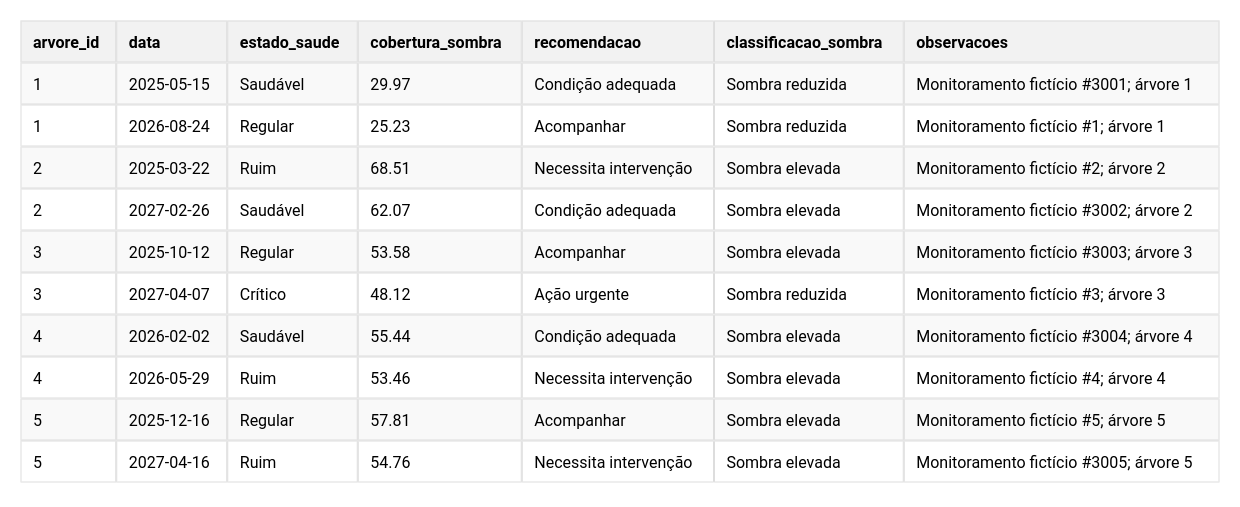
\includegraphics[
            width=\textwidth,
            height=0.8\textheight,
            keepaspectratio]
            {querries_images/modulo_10_funcao_condicionais.png}
        \caption{Tabela gerada com a query}
        \label{fig:consultas_basicas_modulo_10}
    \end{figure}



    \clearpage
    \section*{Módulo 11 (Views)}

    \lstinputlisting[
        language=SQL,
        basicstyle=\ttfamily\tiny,
        caption={Exemplo de Views},
        label={query:modulo_11}
    ]{querries/modulo_11_views.sql}

    \lstinputlisting[
        language=SQL,
        basicstyle=\ttfamily\tiny,
        caption={Exemplo de Views},
        label={query:modulo_11_mostrar}
    ]{querries/modulo_11_views_mostrar.sql}

    \begin{figure}[htbp]
        \centering
        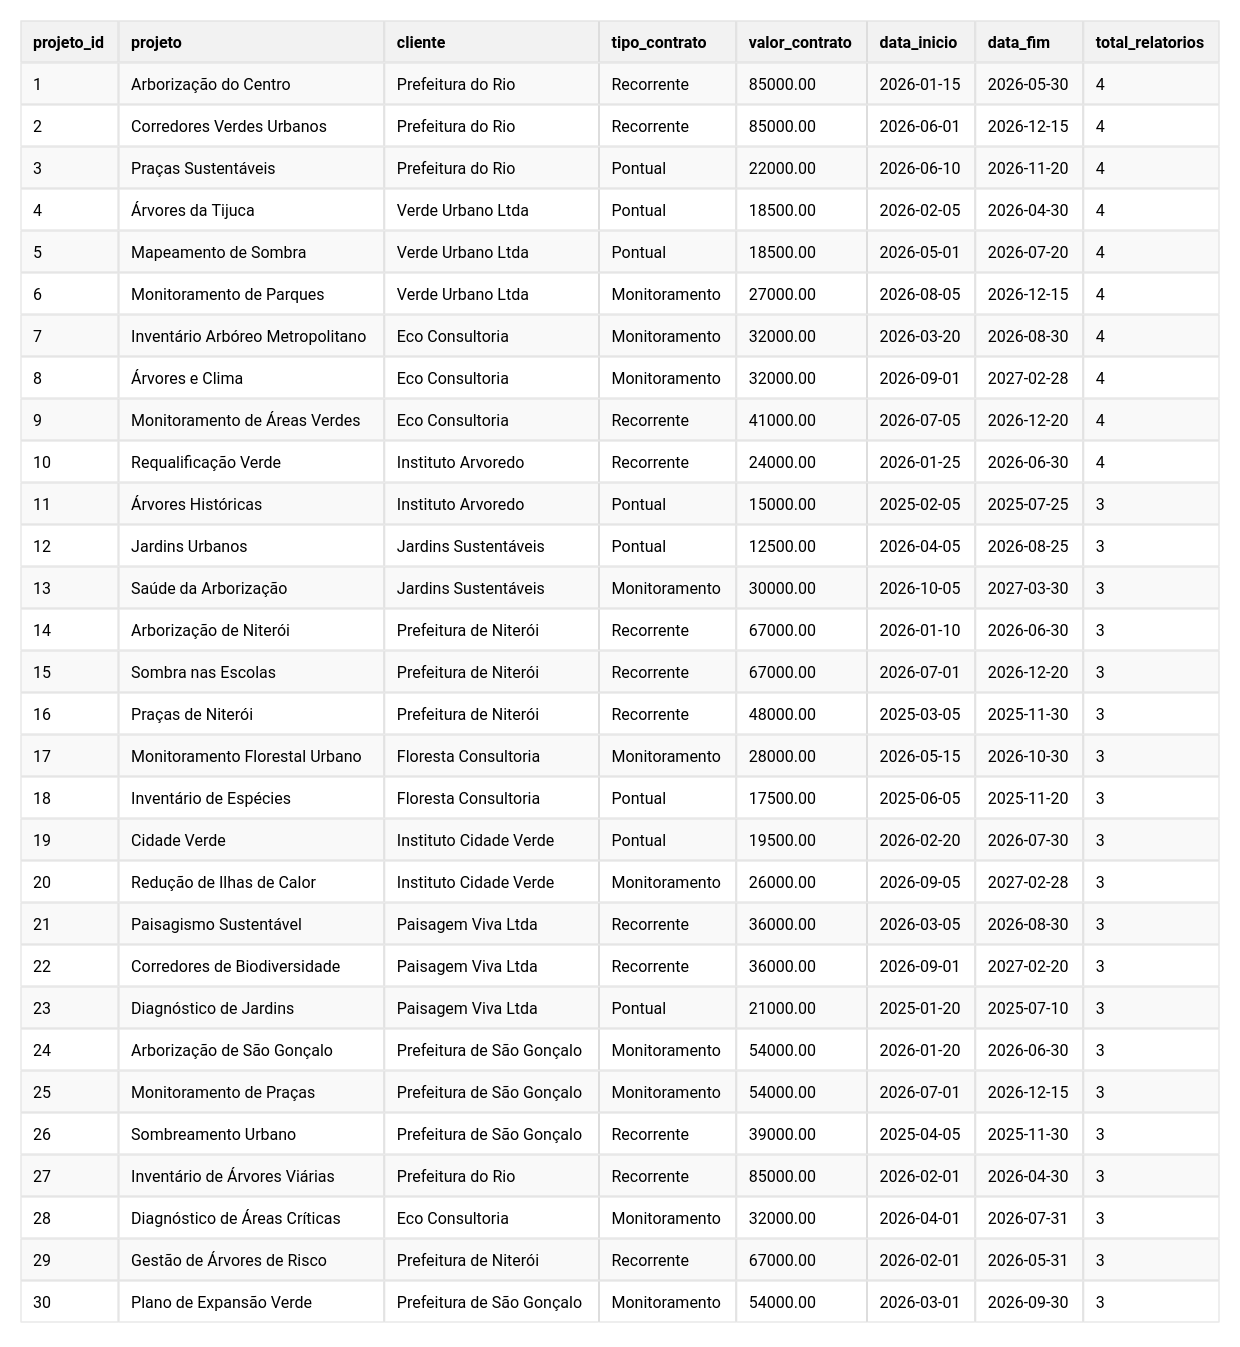
\includegraphics[
            width=\textwidth,
            height=0.4\textheight,
            keepaspectratio]
            {querries_images/modulo_11_views_mostrar.png}
        \caption{Tabela gerada com a query}
        \label{fig:consultas_basicas_modulo_11}
    \end{figure}



    \clearpage
    \section*{Módulo 12 (CRUD / DDL / DML)}

    \lstinputlisting[
        language=SQL,
        basicstyle=\ttfamily\tiny,
        caption={Exemplo de CRUD / DDL / DML},
        label={query:modulo_12}
    ]{querries/modulo_12_crud_ddl_dml.sql}

    \lstinputlisting[
        language=SQL,
        basicstyle=\ttfamily\tiny,
        caption={Exemplo de CRUD / DDL / DML},
        label={query:modulo_12_mostrar}
    ]{querries/modulo_12_crud_ddl_dml_mostrar.sql}

    \begin{figure}[htbp]
        \centering
        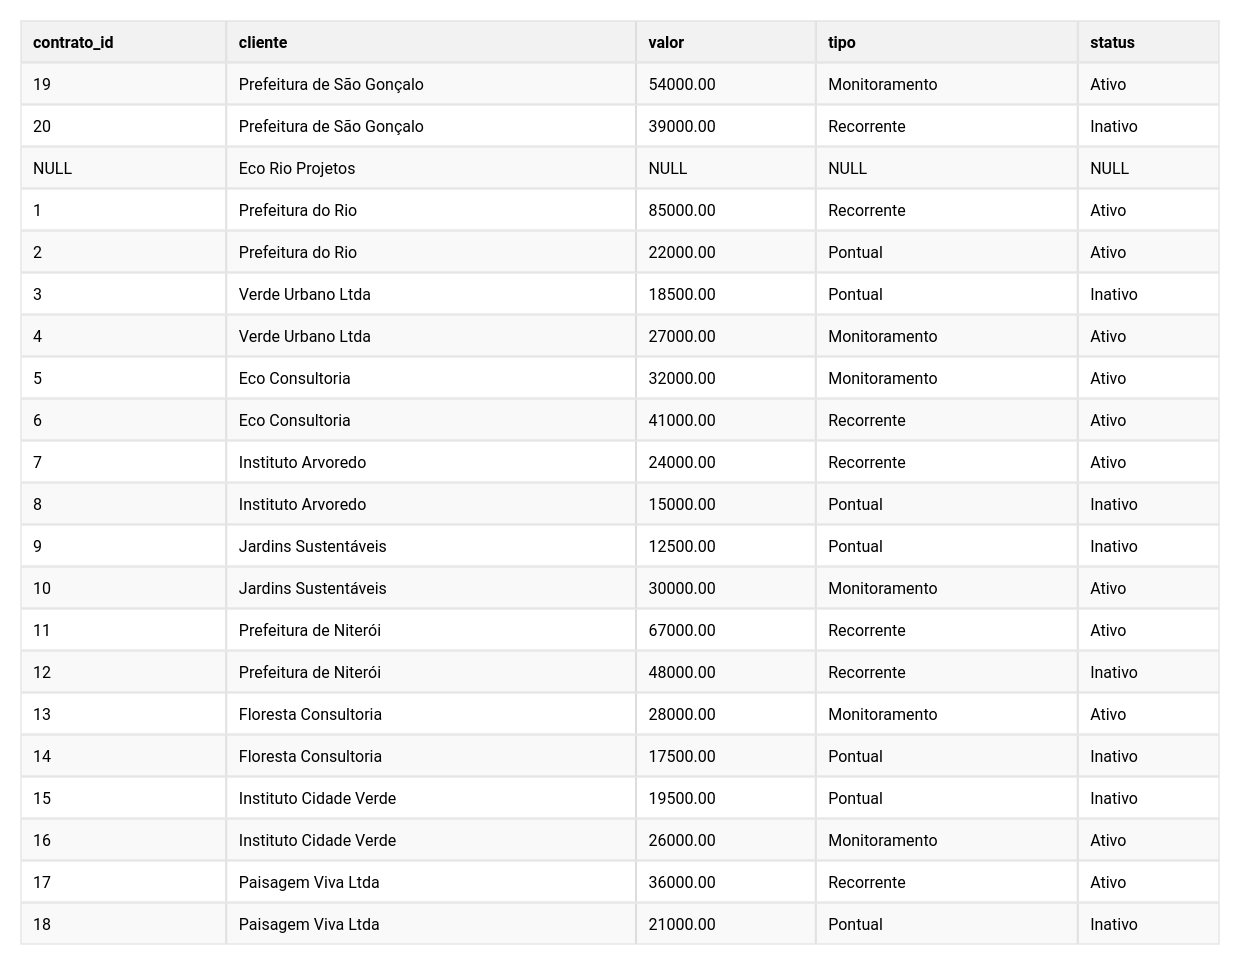
\includegraphics[
            width=\textwidth,
            height=0.4\textheight,
            keepaspectratio]
            {querries_images/modulo_12_crud_ddl_dml_mostrar.png}
        \caption{Tabela gerada com a query}
        \label{fig:consultas_basicas_modulo_12}
    \end{figure}



    \clearpage
    \section*{Módulo 13 (Functions e Procedures)}

    \lstinputlisting[
        language=SQL,
        basicstyle=\ttfamily\tiny,
        caption={Exemplo de Functions},
        label={query:modulo_13_functions}
    ]{querries/modulo_13_functions.sql}

    \begin{figure}[htbp]
        \centering
        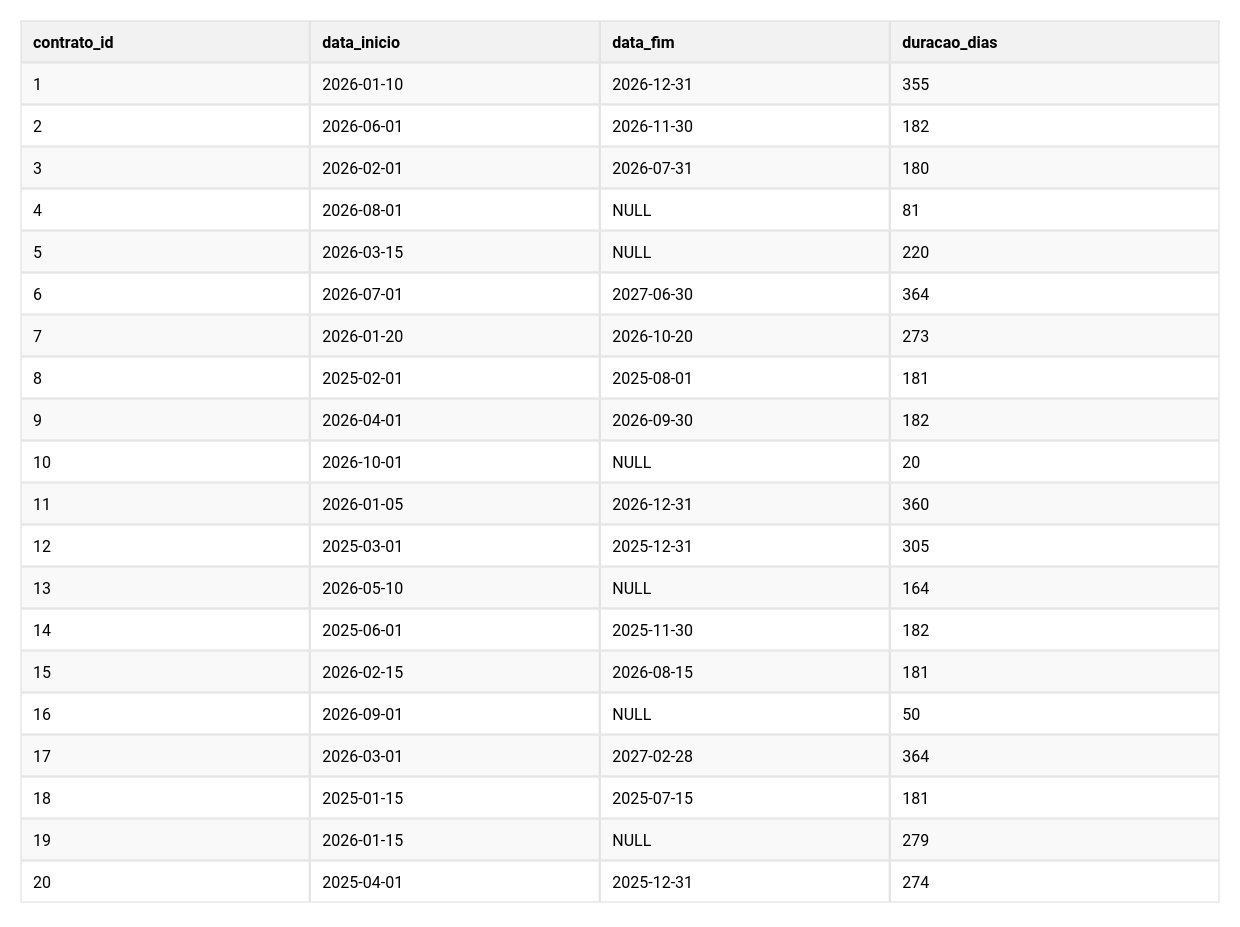
\includegraphics[
            width=\textwidth,
            height=0.8\textheight,
            keepaspectratio]
            {querries_images/modulo_13_functions.png}
        \caption{Tabela gerada com a query}
        \label{fig:consultas_basicas_modulo_13_functions}
    \end{figure}

    \lstinputlisting[
        language=SQL,
        basicstyle=\ttfamily\small,
        caption={Exemplo de Procedures},
        label={query:modulo_13_procedures}
    ]{querries/modulo_13_procedures.sql}

    \begin{figure}[htbp]
        \centering
        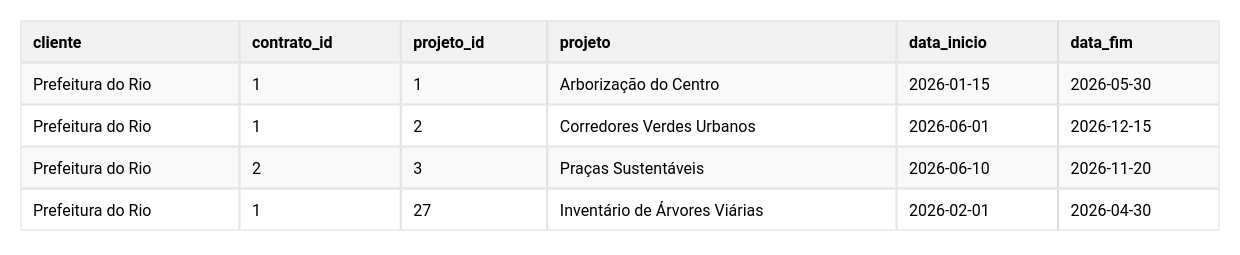
\includegraphics[
            width=\textwidth,
            height=0.8\textheight,
            keepaspectratio]
            {querries_images/modulo_13_procedures.png}
        \caption{Tabela gerada com a query}
        \label{fig:consultas_basicas_modulo_13_procedures}
    \end{figure}

\end{document}